\documentclass[12pt]{amsbook}
\usepackage{preamble}
\newcommand{\vecfieldE}{\boldsymbol{\vec{E}}}
\newcommand{\vecfieldV}{\boldsymbol{\vec{V}}}
\newcommand{\vecfieldU}{\boldsymbol{\vec{U}}}
\newcommand{\rhat}{\boldsymbol{\hat{r}}}
\newcommand{\thetahat}{\boldsymbol{\hat{\theta}}}
\newcommand{\rhohat}{\boldsymbol{\hat{\rho}}}
\newcommand{\vecfieldW}{\boldsymbol{\vec{W}}}
\newcommand{\curvegamma}{\boldsymbol{\vec{\gamma}}}
\newcommand{\tangentgamma}{\boldsymbol{\dot{\vec{\gamma}}}}
\newcommand{\grad}{\boldsymbol{\vec{\nabla}}}
\newcommand{\R}{\mathbb{R}}

\newcommand{\vf}[1]{\boldsymbol{\vec{#1}}}

\begin{document}
\pagenumbering{gobble}       % This kills the page numbering

\begin{center}
   \textsc{\large MATH 272, Exam 1}\\
   \textsc{Oral Examination Problems}\\
   \textsc{Due one hour before your exam time slot.}
\end{center}

\vspace{1cm}

\noindent\textbf{Instructions} \; You are allowed a textbook, homework, notes, worksheets, material on our Canvas page.  You can use online tools such as Desmos and Wolfram Alpha to check your work, but you will need to explain how you arrived at your answers.  You can work with other students and this is, in fact, encouraged! However, I will not be giving out direct help for these problems but can answer questions about previous problems and notes, for example. Ambiguous or illegible answers will not be counted as correct. Scan your solutions and submit them as a pdf on Canvas under Oral Exam 1.  


\vspace{1cm}


\hrule

\vspace*{1cm}
\noindent\emph{Note, there are four total problems.}

\newpage

\begin{problem}
	Let $h(x,y)$ be the height of a sheet above the $xy$-plane at the point $(x,y)$. Then, the level sets of $h$ are exactly the lines you find in a topographic map. Below is a map of White River National Forest, CO including Snowmass Peak. 
	\begin{enumerate}[(a)]
		\item Determine the level set (possibly multiple curves) for $h(x,y)=12,000$.
		\item In the coordinates of this map, the town of Crystal and the famous Crystal Mill is located roughly at $x=18$, $y=25.5$. Locate this point and describe the local geometry (e.g., where the steep and shallow gradients are, which way the river should flow).
		\item Sheep Mountain is located at roughly $x=16.5$ and $y=26$. What is the max elevation of Sheep Mountain?
		\item You want to hike to Snowmass Peak (roughly $(21.5,32)$) because you are very brave. Assuming you are dropped off at Lead King Basin (roughly $(20,28)$). Assuming you can hike over any terrain (including water if need be), can you find a path that follows the steepest gradient from Lead King Basin to Snowmass Peak?
		\item Locate the flattest area that you can.
		\item Plot gradient vectors at each point on the grid.
		\item Follow Schofield Pass starting from roughly $(22.5,19)$. How much elevation gain and loss do you experience over this curve? Can you think of how we could represent this via integration? (\emph{Hint: you may be able to use both $h$ and $\grad h$ to compute this in different ways.})
	\end{enumerate}
\newpage
	\begin{figure}[H]
		\centering
		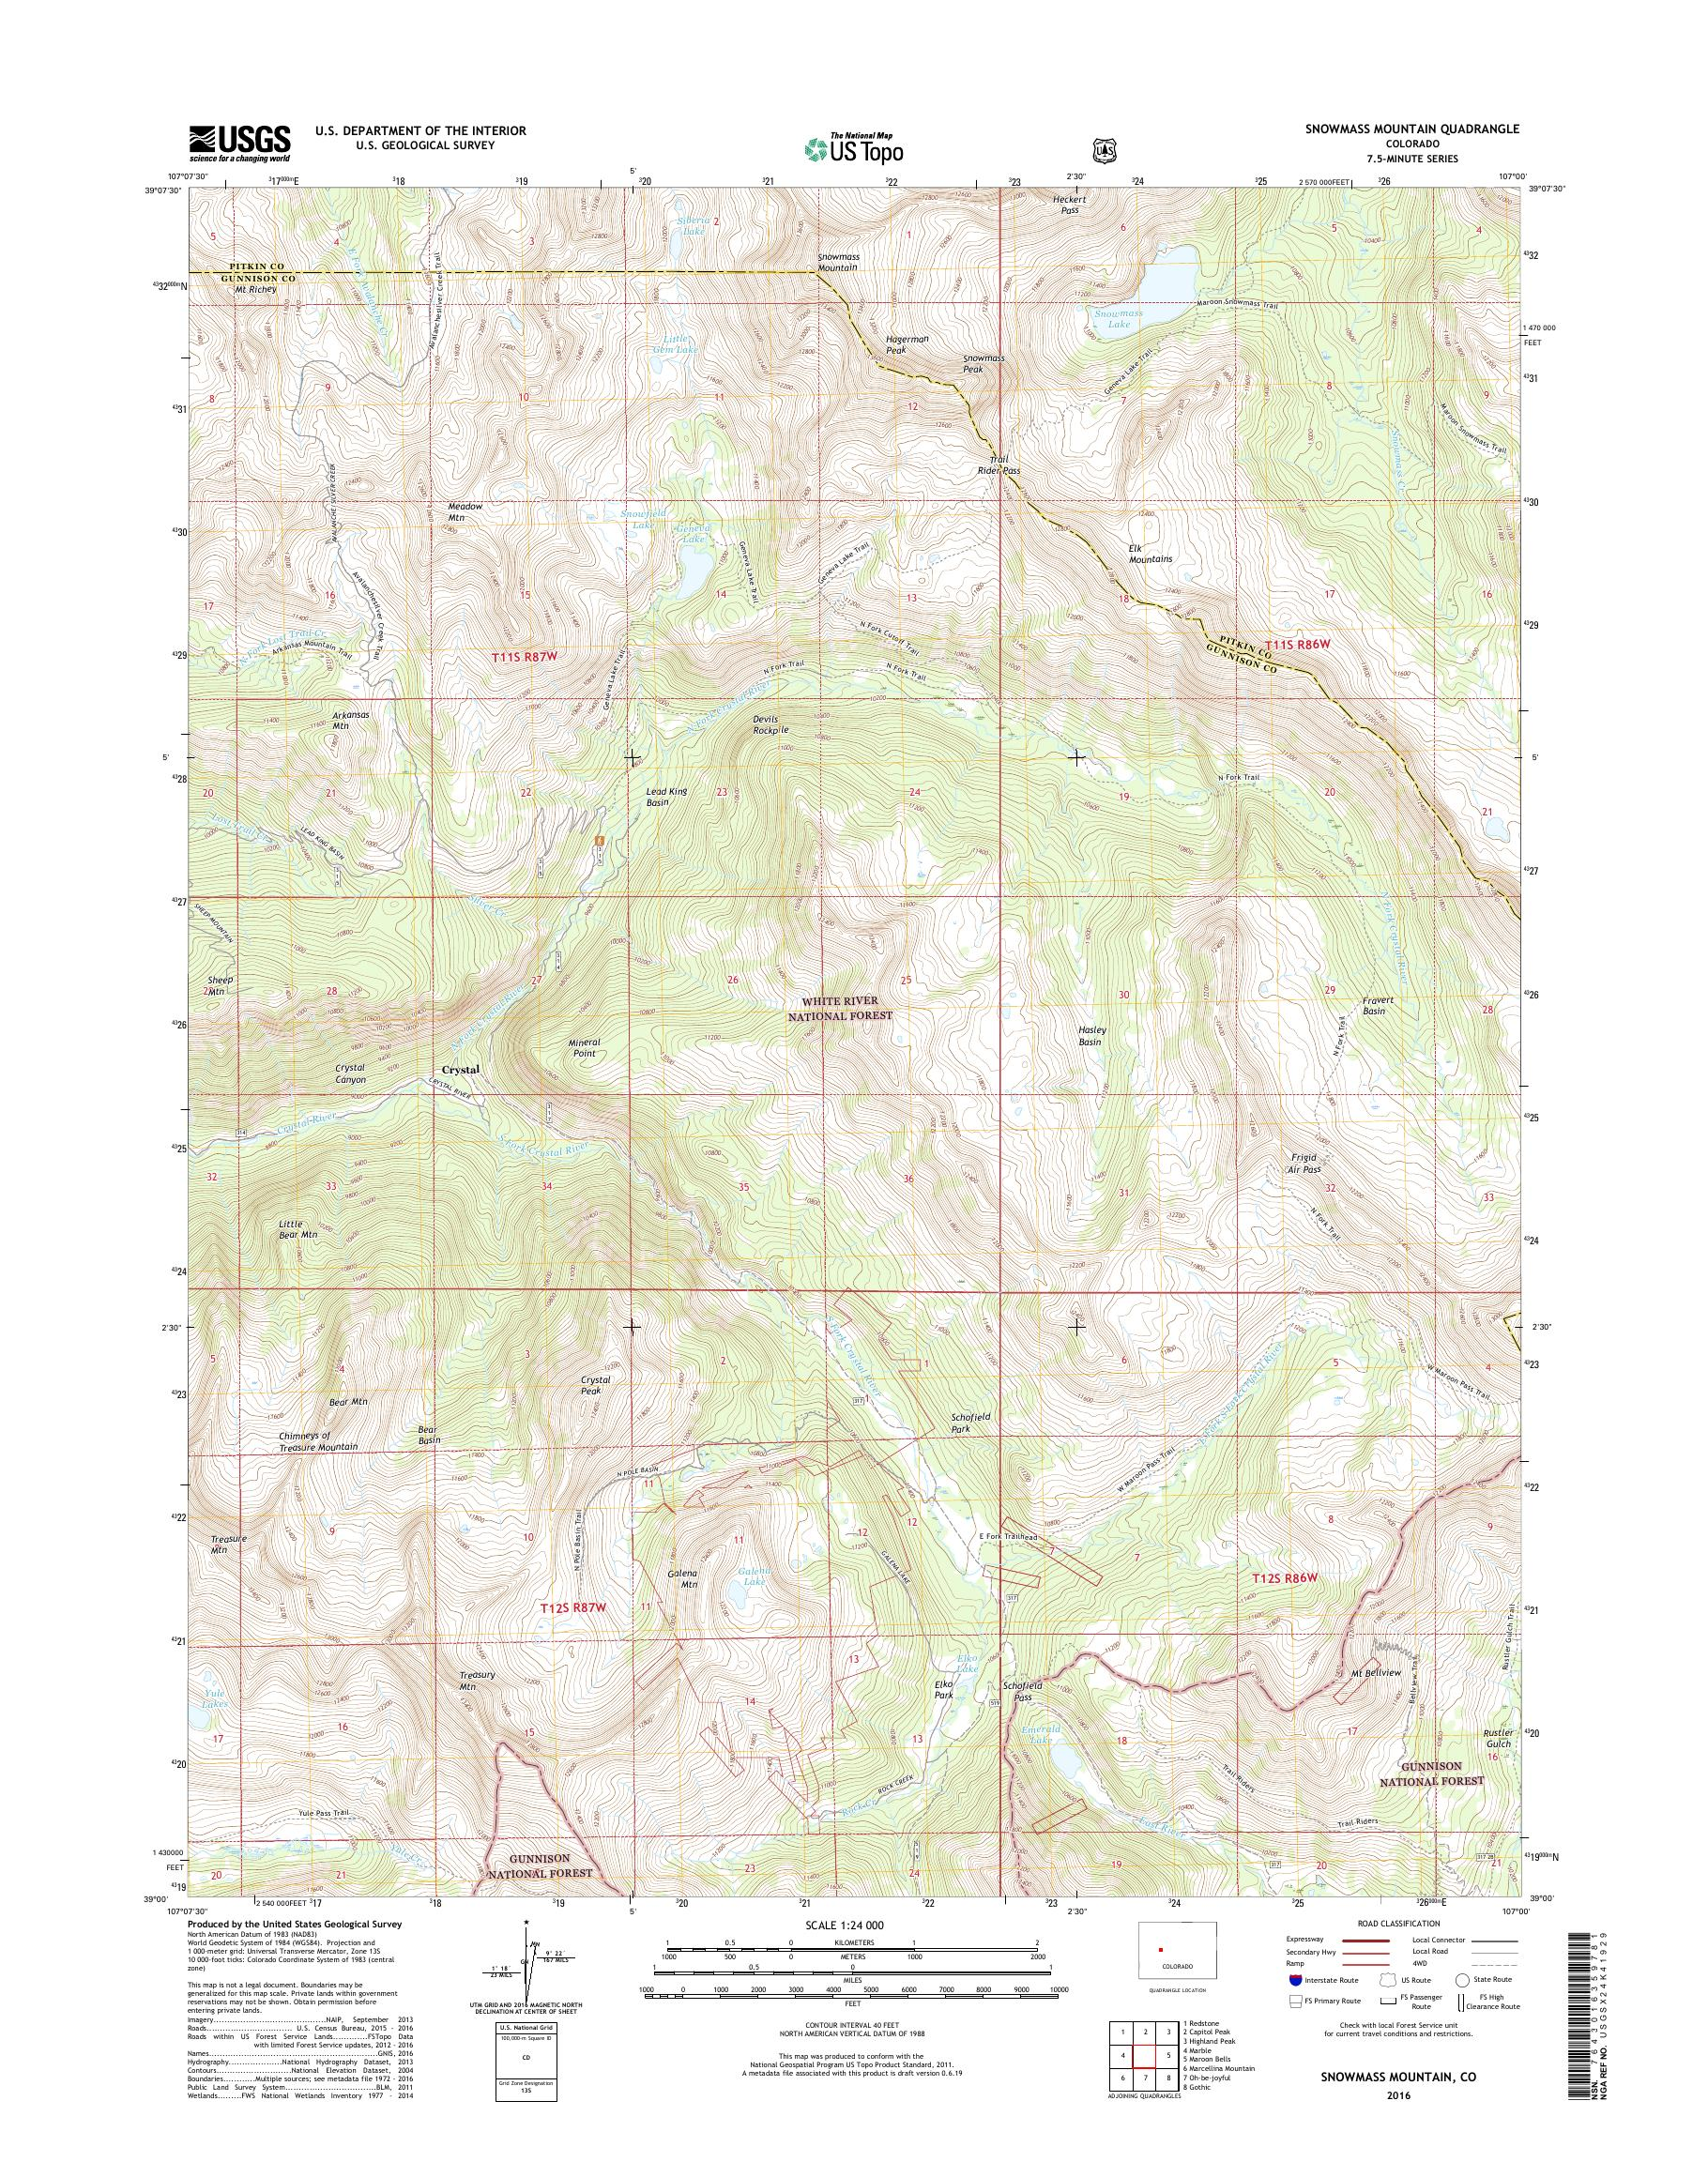
\includegraphics[width=1.2\textwidth]{figures/snowmass_topo.jpg}
	\end{figure}
\end{problem}

\newpage

\begin{problem} A \emph{plasma} is a highly ionized gas. In fact, plasma is the most abundant form of matter in the universe. Plasmas can be treated as charged fluids whose motion is coupled to its own electromagnetic fields.

Because of this, in confined plasmas (e.g., Tokamak \& Stellerator) you may see that the fluid velocity vector field $\vf{v}$ and the fluid vorticity $\vf{\omega}$ are parallel. In other words, $\vf{v}\times \vf{\omega}=0$. 

As a note for plasmas, the vorticity is coupled to the magnetic field and the velocity is coupled to the electric field.

\begin{enumerate}[(a)]
\item Suppose that $\vf{v}$ is the fluid velocity. We say that $\vf{v}$ is a \emph{Beltrami field} if 
\[
\grad \times \vf{v} = \lambda \vf{v}
\]
for some scalar (eigenvalue) $\lambda$. Suppose further that $\vf{v}$ is divergence free, i.e., $\grad \cdot \vf{v}=0$. Show that
\[
\vf{\Delta} \vf{v} = -\lambda^2 \vf{v}
\]
where $\vf{\Delta}$ is the vector Laplacian.
\item Fluid vorticity is the curl of the fluid velocity, i.e., $\vf{\omega} = \grad \times \vf{v}$. Show that if $\vf{v}$ is a Beltrami field, then the fluid vorticity and fluid velocity are parallel.
\item For a specific example, let
\[
\vf{v}(x,y,z) = \begin{pmatrix} \sin(z)+\cos(y) \\ \sin(x)+\cos(z) \\ \sin(y)+\cos(x) \end{pmatrix}.
\]
plot this vector field over a suitable range of input values. 
\item Show that $\vf{v}$ is a Beltrami field. What is the eigenvalue?
\item Show that $\grad \cdot \vf{v}=0$ and find $\vf{\Delta}\vf{v}$ without computing any derivatives.
\end{enumerate}
\end{problem}

\newpage
\begin{problem}
Consider a curve 
\[
\curvegamma(t) = \begin{pmatrix} \cos(t) \\ \sin(t) \\ \cos(2t) \end{pmatrix} \qquad t\in [0,2\pi].
\]
Imagine this curve is a wire that we dip into a soapy solution. What will the shape of the bubble that forms on this wire look like? Let's work through it.
        \vspace*{0.25cm}
    \begin{enumerate}[(a)]
        \item Consider the function $f(x,y)=x^2-y^2$. Plot the graph of this function and the curve $\curvegamma$ simultaneously.
        \vspace*{0.25cm}
        \item Show that for points $(x,y)$ on the unit circle in the $xy$-plane that the graph of $f(x,y)$ matches the points along $\curvegamma$. \emph{Hints:}
        \begin{itemize}
        \item \emph{You should be able to see this in your plot from (a). This isn't proof, but it can help you visualize the problem.}
        \item \emph{Can you parameterize the unit circle as a curve $\boldsymbol{\vec{\eta}}(t)$ and consider $f(\boldsymbol{\vec{\eta}}(t))$?}
        \end{itemize}
        \vspace*{0.25cm}
        \item Show that $f(x,y)$ is harmonic. That is, show $\Delta f = 0$. This shows the bubble is a \emph{minimal surface}.
        \vspace*{0.25cm}
        \item Set up the integral 
        \[
        \int_\Sigma d\Sigma,
        \]
        which computes the area of the soap film. Here, $\Sigma$ is the graph of the function $f(x,y)$ with the domain given by the unit disk $x^2+y^2\leq 1$.
        \vspace*{0.25cm}
        \item \textrm{(BONUS)} Convert the integral in the previous part to cylindrical coordinates and find a numerical value for the integral. \emph{You will not be able to get WolframAlpha to compute this integral in cartesian coordinates -- this is another reason why using coordinate systems better suited to your problem is important!}
    \end{enumerate}
\end{problem}

\newpage
\begin{problem} Let us explore our other coordinate systems.
    \begin{enumerate}[(a)]
        \item Define a function in cylindrical coordinates that is constant on the surface of an infinitely tall cylinder of radius 1 but is not constant in all of space.
        \vspace*{0.25cm}
        \item Set up the bounds of an integral in spherical coordinates that integrates over an eighth of a thick spherical shell with inner radius 5 and outer radius 25. Take the eighth that lies in the octant where $x$ and $y$ are both positive.
        \vspace*{0.25cm}
        \item Convert the following function 
        \[
        f(x,y,z) = \frac{x}{y(x^2+y^2+z^2)}
        \]
        into spherical coordinates.
    \end{enumerate}
\end{problem}



\end{document}  